%==============================================================================
\section{Background and Problem Definition}
\label{sec:background}

\subsection{Property Graph Model}
\label{sec:background:graph}


\noindent\textit{\textbf{Data Model.}} A \emph{property graph} $G = (V, E)$ consists of a set of nodes $V$ and a set of directed 
edges $E \subseteq V \times V$. We adopt the property graph model~\cite{robinson2015graph}, 
which represents data using nodes, edge relationships, and associated properties.

\begin{itemize}[leftmargin=*]
\item {Node:} Nodes represent entities in the graph and are grouped by \textit{labels}, 
which denote node types. Within each label, individual nodes are uniquely identified by an id.

\item {Edge relationship:} Edges capture directed connections between nodes 
    of the same or different labels, and are identified by an \emph{edge 
    label}. Each edge connects a source node to a destination node; we restrict any pair of nodes to at most one edge of a given label.

\item {Property:} Nodes and edges can each be associated with a set of properties that store additional descriptive attributes.
\end{itemize}


\noindent\textit{\textbf{Storage Model.}} 
Existing oblivious database storage models translate poorly to graph data. Most oblivious database systems store data either in a key-value format 
~\cite{dauterman2021snoopy, mishra2018oblix} or in a row-oriented tabular 
format~\cite{zheng2017opaque,eskandarian2019oblidb,mavrogiannakis2025obliviator}. For example, 
GraphOS~\cite{chamani2023graphos} stores graph data as key-value pairs in an oblivious AVL tree, 
incurring $O(\mathrm{polylog}\,N)$ overhead \emph{per node or edge access}, incurring prohibitive overheads for million-scale graphs. Row-wise tables fare no better for 
analytical workloads. \system instead uses a disk-based \emph{columnar} layout where
each node and edge property occupies a separate column file, with properties 
that are commonly queried together stored together for efficient access.


Unlike plaintext \gdbs, oblivious \gdbs require careful consideration in how to store the
edge lists. Simply storing node-edge relationship in an adjacency list reveals the degree of 
each node even if node and edge ids are encrypted. Hiding node degrees would require padding 
each entry to a worst-case size of $m \times n$, where $m$ denotes the number of edges and $n$ 
the number of nodes, since in the worst case all $m$ edges may originate from a single node.
To avoid this leakage, we instead store adjacency information in a single array-like structure 
sorted by source node ids, thus only revealing the total number of edges $m$ (for a given edge 
label), which we treat as non-sensitive.

Furthermore, following common design practices in plaintext \gdbs such 
as~\cite{janusgraph,feng2023kuzu,deutsch2019tigergraph,sun2015sqlgraph}, we also maintain 
\textit{reverse edges}, stored in sorted order of destination node ids. This reverse index of 
size $m$ enables efficient bidirectional traversal and parallel processing of graph 
queries. 


\noindent\textbf{\textit{Query Model.}} \system supports Cypher-like queries~\cite{francis2018cypher, opencypher} in 
which each query specifies a node-edge pattern to match and predicates to 
filter on properties. We distinguish two types of acyclic queries:

\begin{itemize}[leftmargin=*]
    \item A \textbf{one-hop query} matches two nodes connected by an edge: (source node) $\rightarrow$ [edge] $\rightarrow$ (destination node). For example, ``find all transactions from accounts with balance $>$ 10000'':
    \begin{center}
    \texttt{(a:Account)-[t:Transaction]$\rightarrow$(b:Account)}\\
    \texttt{WHERE a.balance > 10000}
    \end{center}

    \item A \textbf{$k$-hop query} chains $k+1$ nodes traversing $k$ edges. For example, a 3-hop query might find ``accounts reachable within 3 transactions from a flagged account'':
    \begin{center}
    \small\texttt{(a1:Account)-[t1:Transaction]$\rightarrow$(a2:Account)-[t2:Transaction]\\
    $\rightarrow$}\small\texttt{(a3:Account)-[t3:Transaction]$\rightarrow$(a4:Account)}
    \end{center}
\end{itemize}

The output contains all nodes and edges satisfying both the structural pattern 
and the predicates. In relational terms, a $k$-hop query is a $(2k+1)$-way 
join over $k+1$ node tables and $k$ edge tables, joined on foreign key 
relationships, with predicate filters potentially applied at each node and edge table.
%------------------------------------------------------------------------------
\subsection{System and Threat Model}
\label{sec:background:threat}
%------------------------------------------------------------------------------
We consider a system model where an organization outsources its storage and computational needs to a 
cloud. The organization uploads encrypted graph data to the cloud and issues queries to \system hosted
within a Trusted Execution Environment (TEE) such as Intel TDX~\cite{intel_tdx}, AMD SEV-SNP~\cite{sev2020strengthening}. The TEE provides hardware-enforced 
isolation: code and data inside the enclave are protected from the host OS, 
hypervisor, and other software via an encryption engine keyed to a 
processor-embedded root key. Remote attestation allows clients to verify the 
integrity of the software running inside the TEE.

\system adopts the semi-honest attacker model common in enclave-based 
systems~\cite{dauterman2021snoopy, krastnikov2020efficient, mishra2018oblix, 
chamani2023graphos, mavrogiannakis2025obliviator}: the adversary observes 
encrypted network traffic, controls the software stack outside the enclave, 
and monitors memory accesses at cache-line granularity, but cannot breach the 
secure processor or access its secret key. This exposes the system to 
side-channel attacks including cache attacks~\cite{brasser2017software, 
hahnel2017high, moghimi2017cachezoom, schwarz2017malware}, branch prediction 
and page-fault attacks~\cite{lee2017inferring, van2017telling, xu2015controlled}, 
and memory bus snooping~\cite{lee2020off}. Power and timing attacks are out 
of scope.

This model differs from trusted-proxy oblivious 
systems~\cite{ahmed2025oasisdb, demertzis2020seal, li2014fast, 
chang2022towards, chang2021efficient}, where the adversary has no visibility 
into the proxy machine running the obliviousness scheme. Those \emph{singly} 
oblivious schemes need only hide data access patterns from storage. In the 
TEE setting, where the adversary monitors memory inside the enclave itself, 
the scheme must additionally obfuscate its own memory access pattern and 
control flow, forming the \emph{doubly} oblivious requirement that \system is 
designed to satisfy.

\subsection{Security Definition}
\label{sub:sec-definition}

An algorithm is \emph{oblivious} if its externally observable behavior is 
independent of its input data, beyond a defined set of permitted leakage. 
Concretely, for any two inputs consistent with the same public parameters and 
producing outputs of the same size, an adversary observing execution should be 
unable to determine which input was used. For \system, this means that 
observable side channels --- logical data accesses (e.g., which node entries 
are read), physical memory access patterns (e.g., which cache lines are 
touched), and control flow decisions --- must be independent of both the 
underlying graph data and the query predicates.

We formalize this via a simulation-based definition, which captures the 
intuition that everything an adversary learns from observing execution could 
have been produced without access to the data. Let $\mathcal{L}$ denote the 
permitted leakage. In \system, $\mathcal{L}$ comprises the graph schema, the 
base table sizes for node and edge labels referenced by the query, the query 
structure, and the final result size. Crucially, intermediate result sizes,
which prior join-based schemes~\cite{ruidi2025oblivious, 
mavrogiannakis2025obliviator} may expose, are \emph{not} part of 
$\mathcal{L}$ and must be hidden.

We define a security game in which an execution trace is generated either by 
the real algorithm $\mathsf{Alg}$ or by a PPT simulator $\mathsf{Sim}$ given 
only $\mathcal{L}$. The algorithm is oblivious if no PPT adversary 
$\mathcal{A}$ can distinguish between the two with more than negligible 
advantage.

\begin{definition}
\label{def:oblivious}
An algorithm $\mathsf{Alg}$ is \emph{oblivious} with respect to leakage 
$\mathcal{L}$ if there exists a PPT simulator $\mathsf{Sim}$ such that for 
all PPT adversaries $\mathcal{A}$:
\[
\left| 
\Pr\left[\mathcal{A}(\mathsf{Trace}_{\mathsf{Alg}}) = 1\right] 
- 
\Pr\left[\mathcal{A}(\mathsf{Sim}(\mathcal{L})) = 1\right] 
\right| \leq \mathrm{negl}(\lambda),
\]
where $\lambda$ is the security parameter and $\mathsf{Trace}_{\mathsf{Alg}}$ 
denotes the observable execution trace of $\mathsf{Alg}$.
\end{definition}
\subsection{Oblivious Primitives}
\label{sub:obl-primitives}

\system leverages a number of oblivious primitives as building blocks, which we describe next.

\noindent\textbf{Oblivious compare and set (\textsc{OCmpSet}):}  
A key requirement for oblivious execution is to eliminate secret-dependent branching,
since conditional control flow may leak information through execution traces.  
Instead, we express conditionals using data-independent bitwise operations that can be
efficiently realized using SIMD instructions.  
Given a secret predicate \texttt{flag}, \textsc{OCmpSet}(\texttt{flag}, $x$, $y$) selects $x$ if \texttt{flag}
is true and otherwise $y$, without revealing the value of \texttt{flag} and whether $x$ or $y$ was selected.

\noindent\textbf{Oblivious sorting (\textsc{OSort}):}  
Oblivious sorting rearranges an input array into sorted order while ensuring that the
sequence of comparisons and memory accesses is independent of the input values.
\system adopts bitonic sorting \cite{batcher1968sorting} due to its deterministic structure and 
strong parallelization properties. Bitonic sort executes a fixed sequence of compare-exchange
operations, yielding a time complexity of $O(n \log^2 n)$ for input size $n$, and
$O((n \log^2 n)/p)$ when parallelized across $p$ threads.  
While asymptotically optimal $O(n \log n)$ oblivious sorting algorithms exist ~\cite{ajtai1983sorting, 
goodrich2014zigzag, gu2025flexway}, they often incur higher constants or exhibit limited scalability when
parallelized~\cite{ngai2024distributed}.  

\noindent\textbf{Oblivious compaction (\textsc{OCompact}):}  
Oblivious compaction takes an array of $n$ elements, each annotated with a binary
predicate (e.g., marked or unmarked), and produces a permutation in which all marked
elements are grouped together while preventing any leakage through memory traces.  
Although linear-time compaction algorithms exist \cite{dittmer2020oblivious,goodrich2011oblivious},
they are often difficult to parallelize and incur high constant overheads. Instead, we use 
ORCompact~\cite{sasy2022fast}, which achieves $O(n \log n)$ complexity while enabling parallel execution.  
ORCompact additionally preserves the relative order of marked elements.

\noindent\textbf{Oblivious hash table (\textsc{OHashTable}):}
An oblivious hash table supports key-value \textsf{build} and 
\textsf{lookup} operations such that the memory access pattern of each 
operation is independent of the keys queried or the distribution of 
values. Concretely, \textsf{build} takes $n$ key-value pairs and 
constructs the table; and \textsf{lookup} accepts a key (or a 
dummy) and returns the associated value or $\bot$, without revealing 
whether the key was present. We use the oblivious hash table of 
H2O2RAM~\cite{zheng2025h2o2ram}, which selects among three schemes 
--- bucket hash, stashless Cuckoo hash, and two-tier hash --- depending 
on table size and lookup frequency. Build complexity ranges from 
$O(n\log^2 n)$ for small to moderate tables to $O(n\log^2\log n)$ for large 
tables, and lookup runs in $O(\ell)$ time where $\ell$ is the bucket size. 
\textsc{OHashTable} requires that all input entries passed to 
\textsf{build} have distinct keys, and that no key is submitted to 
\textsf{lookup} more than once.


\subsection{Oblivious Multi-Way Joins}
\label{sec:background:joins}

\begin{figure}
    \centering
    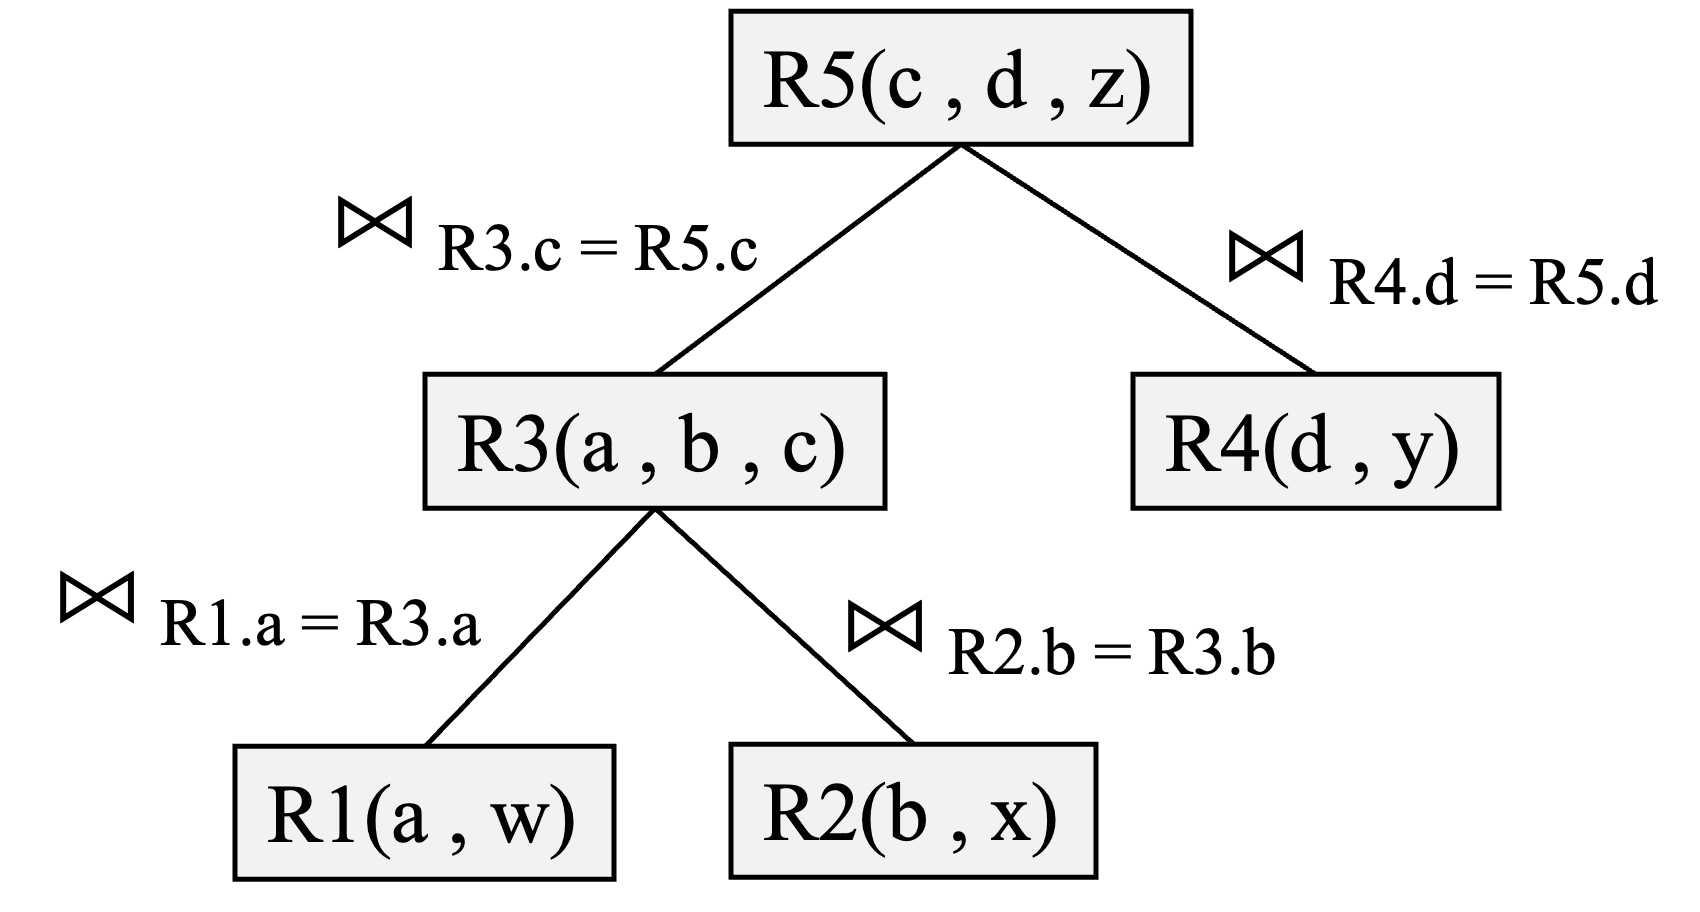
\includegraphics[width=0.5\linewidth]{figures/multi-way-join.png}
    \caption{A multi-way join tree of relations $R_1$ to $R_5$.}
    \label{fig:multiway-join}
\end{figure}

\system builds on the oblivious multi-way join algorithm of Wei and
Kerschbaum~\cite{ruidi2025oblivious}, referred to as \wei. Given $k$
relations $R_1, \ldots, R_k$ whose join predicates form an acyclic join
graph, \wei evaluates $R_1 \bowtie \cdots \bowtie R_k$ by constructing a
join tree (Figure~\ref{fig:multiway-join}). Concretely, \wei's access
pattern depends only on the sizes of the input relations and the final
join output size --- no intermediate result size is ever revealed.

The key abstraction is \emph{multiplicity}: rather than materializing
intermediate join results, \wei computes for every tuple $t$ a single
integer $\alpha_{\mathit{final}}(t)$: the number of rows in the final
result in which $t$ participates. Once these are known, it produces
the final output by replicating each tuple $\alpha_{\mathit{final}}(t)$
times and aligns the copies. The entire difficulty reduces to computing
multiplicities obliviously.

\Wei does this in two phases over the join tree. In the \textbf{bottom-up}
phase, each tuple is first assigned a \emph{local multiplicity}
$\alpha_{\mathit{local}}$: the number of partial results it participates
in within the subtree rooted at its relation. Leaf tuples start at
$\alpha_{\mathit{local}} = 1$. For each parent-child pair, it concatenates
the two relations and obliviously sorts them on the join attribute,
grouping tuples with matching keys. A linear scan aggregates, for each
parent tuple, the sum of local multiplicities of all matching child
tuples; the parent's local multiplicity is the product of contributions
across all its children. At the root, $\alpha_{\mathit{local}}$
equals $\alpha_{\mathit{final}}$ directly, since the root's subtree
is the entire tree.

The \textbf{top-down} phase propagates $\alpha_{\mathit{final}}$ from
the root downward using the same concatenate-sort-scan machinery in
reverse, combining each tuple's local multiplicity with the contribution
from outside its subtree. With all final multiplicities known, \wei
materializes the output in three steps: \emph{(i) expansion}, replicating
each tuple $\alpha_{\mathit{final}}$ times; \emph{(ii) alignment},
ordering matching tuples consistently across relations; and \emph{(iii)
merge}, combining aligned tuples into the final result.


The overall complexity is $O(N \log N + \mathit{OUT})$, where $N$ is the total 
input size and $\mathit{OUT}$ is the output size. \sujaya{@Bishwajit: Shouldn't there be a sort on the output size??} The dominant concrete cost is 
oblivious sorting: each parent-child pair requires six sorts, three per 
phase. \system reduces this cost by decomposing multi-hop queries to minimize 
join tree depth, as described in Section~\ref{sec:onehop}.